\chapter{Tabeller og figurer} \label{app:data}
Dette appendiks indeholder nogle tabeller og figurer, som anvendes i den empiriske del. 

%%%%%%% AR(4) %%%%%%%

%\imgfigh{descrip_ar.pdf}{0.7}{Analyse af de standardiserede residualer for AR(4). }{resid_ar}

%%%%%%% Faktor modellen %%%%%%%

\imgfigh{ic1_res.pdf}{0.7}{Analyse af de standardiserede residualer for faktor modellen valgt udfra IC$_1$. }{ic1_res}
%
\imgfigh{ic2_res.pdf}{0.7}{Analyse af de standardiserede residualer for faktor modellen valgt udfra IC$_2$. }{ic2_res}

%%%%%%% Krydsvalidering %%%%%%%

\imgfigh{resid_lasso_coord_kryds.pdf}{0.7}{Analyse af de standardiserede residualer for lasso model med optimeringsmetoden coodinate descent, hvor krydsvalidering er brugt til at estimere $\widehat{\lambda}$. }{resid_lasso_coord_kryds}

\imgfigh{resid_ridge_coord_kryds.pdf}{0.7}{Analyse af de standardiserede residualer for ridge regression med optimeringsmetoden coodinate descent, hvor krydsvalidering er brugt til at estimere $\widehat{\lambda}$. }{resid_ridge_coord_kryds}

\imgfigh{resid_grp_coord_kryds.pdf}{0.7}{Analyse af de standardiserede residualer for group lasso med optimeringsmetoden coodinate descent, hvor krydsvalidering er brugt til at estimere $\widehat{\lambda}$. }{resid_grp_coord_kryds}

\imgfigh{resid_adap_ols_coord_kryds.pdf}{0.7}{Analyse af de standardiserede residualer for adaptive lasso med ols vægte med optimeringsmetoden coodinate descent, hvor krydsvalidering er brugt til at estimere $\widehat{\lambda}$. }{resid_adap_ols_coord_kryds}

\imgfigh{resid_adap_lasso_coord_kryds.pdf}{0.7}{Analyse af de standardiserede residualer for adaptive lasso med lasso vægte med optimeringsmetoden coodinate descent, hvor krydsvalidering er brugt til at estimere $\widehat{\lambda}$. }{resid_adap_ols_coord_kryds}
\begin{sidewaystable} 
%\begin{table}
\center
\scalebox{0.8}{
\begin{tabular}{lccccccccccc} 
Krydsvalidering\\
\toprule
& Lasso (CV) && Ridge regression (CV) && Group lasso  (CV) && Adap. lasso m. OLS vægte (CV)  && Adap. lasso m. lasso vægte (CV) & Lasso$_{TG}$ (CV)  \\ \midrule
Skewness & $-0.1610$ &&$-0.1194$ && $-0.0943$ & &   $-0.1167$ && $-0.1134$  & -0.0964\\
Kurtosis & $ -0.4633 $ && 0.5568 &&  $-0.3725$ &&    $-0.5186$ && $-0.5429$ & -0.5201 \\
JB-test & 0.0289 && 0.0128 &&  0.1478  &&  0.0118 &&  0.0214 & 0.0331\\
LB$_{10}$-test &  0  && 0.0017 && 0  &&  0&  & 0 & 0 \\ \bottomrule \toprule
BIC\\ \midrule
& Lasso (BIC) && Ridge regression (BIC) &&Group lasso (BIC) &  & Adap. lasso m. OLS vægte (BIC)&& Adap. lasso m. lasso  vægte (BIC) &  Lasso$_{TG}$ (BIC)   \\ \midrule
Skewness &$-0.1322$ && $-0.1127$ && $-0.1148$ & & $-0.0869$ && $-0.0912$ & 0.0935  \\
Kurtosis & $-0.5174$ && 0.5124 &&$-0.2385$ && $-0.6104$ && $-0.5994$ & -0.5310 \\
JB-test & 0.0235 && 0.0239 && 0.3008   &&   0.0113 &&$0.0127$ & 0.0298  \\
LB$_{10}$-test & 0 &&  0.0013 && 0  &  & 0 &&  0 & 0 \\  \bottomrule
 \end{tabular}}
\caption{Skewness, excess kurtosis og \(p\)-værdier for Jarque Bera og Ljung Box testen for de standardiserede residualer fra shrinkage metorderne, hvor $\widehat{\lambda}$ er valgt udfra krydsvalidering og BIC. Vi lader LB$_{10}$ betegne Ljung-Box testen med lag = 10. } \label{tab:res_shrinkage_tab}
%\end{table}
\end{sidewaystable}


\begin{landscape}
\begin{figure}[htbp]
		\centering
		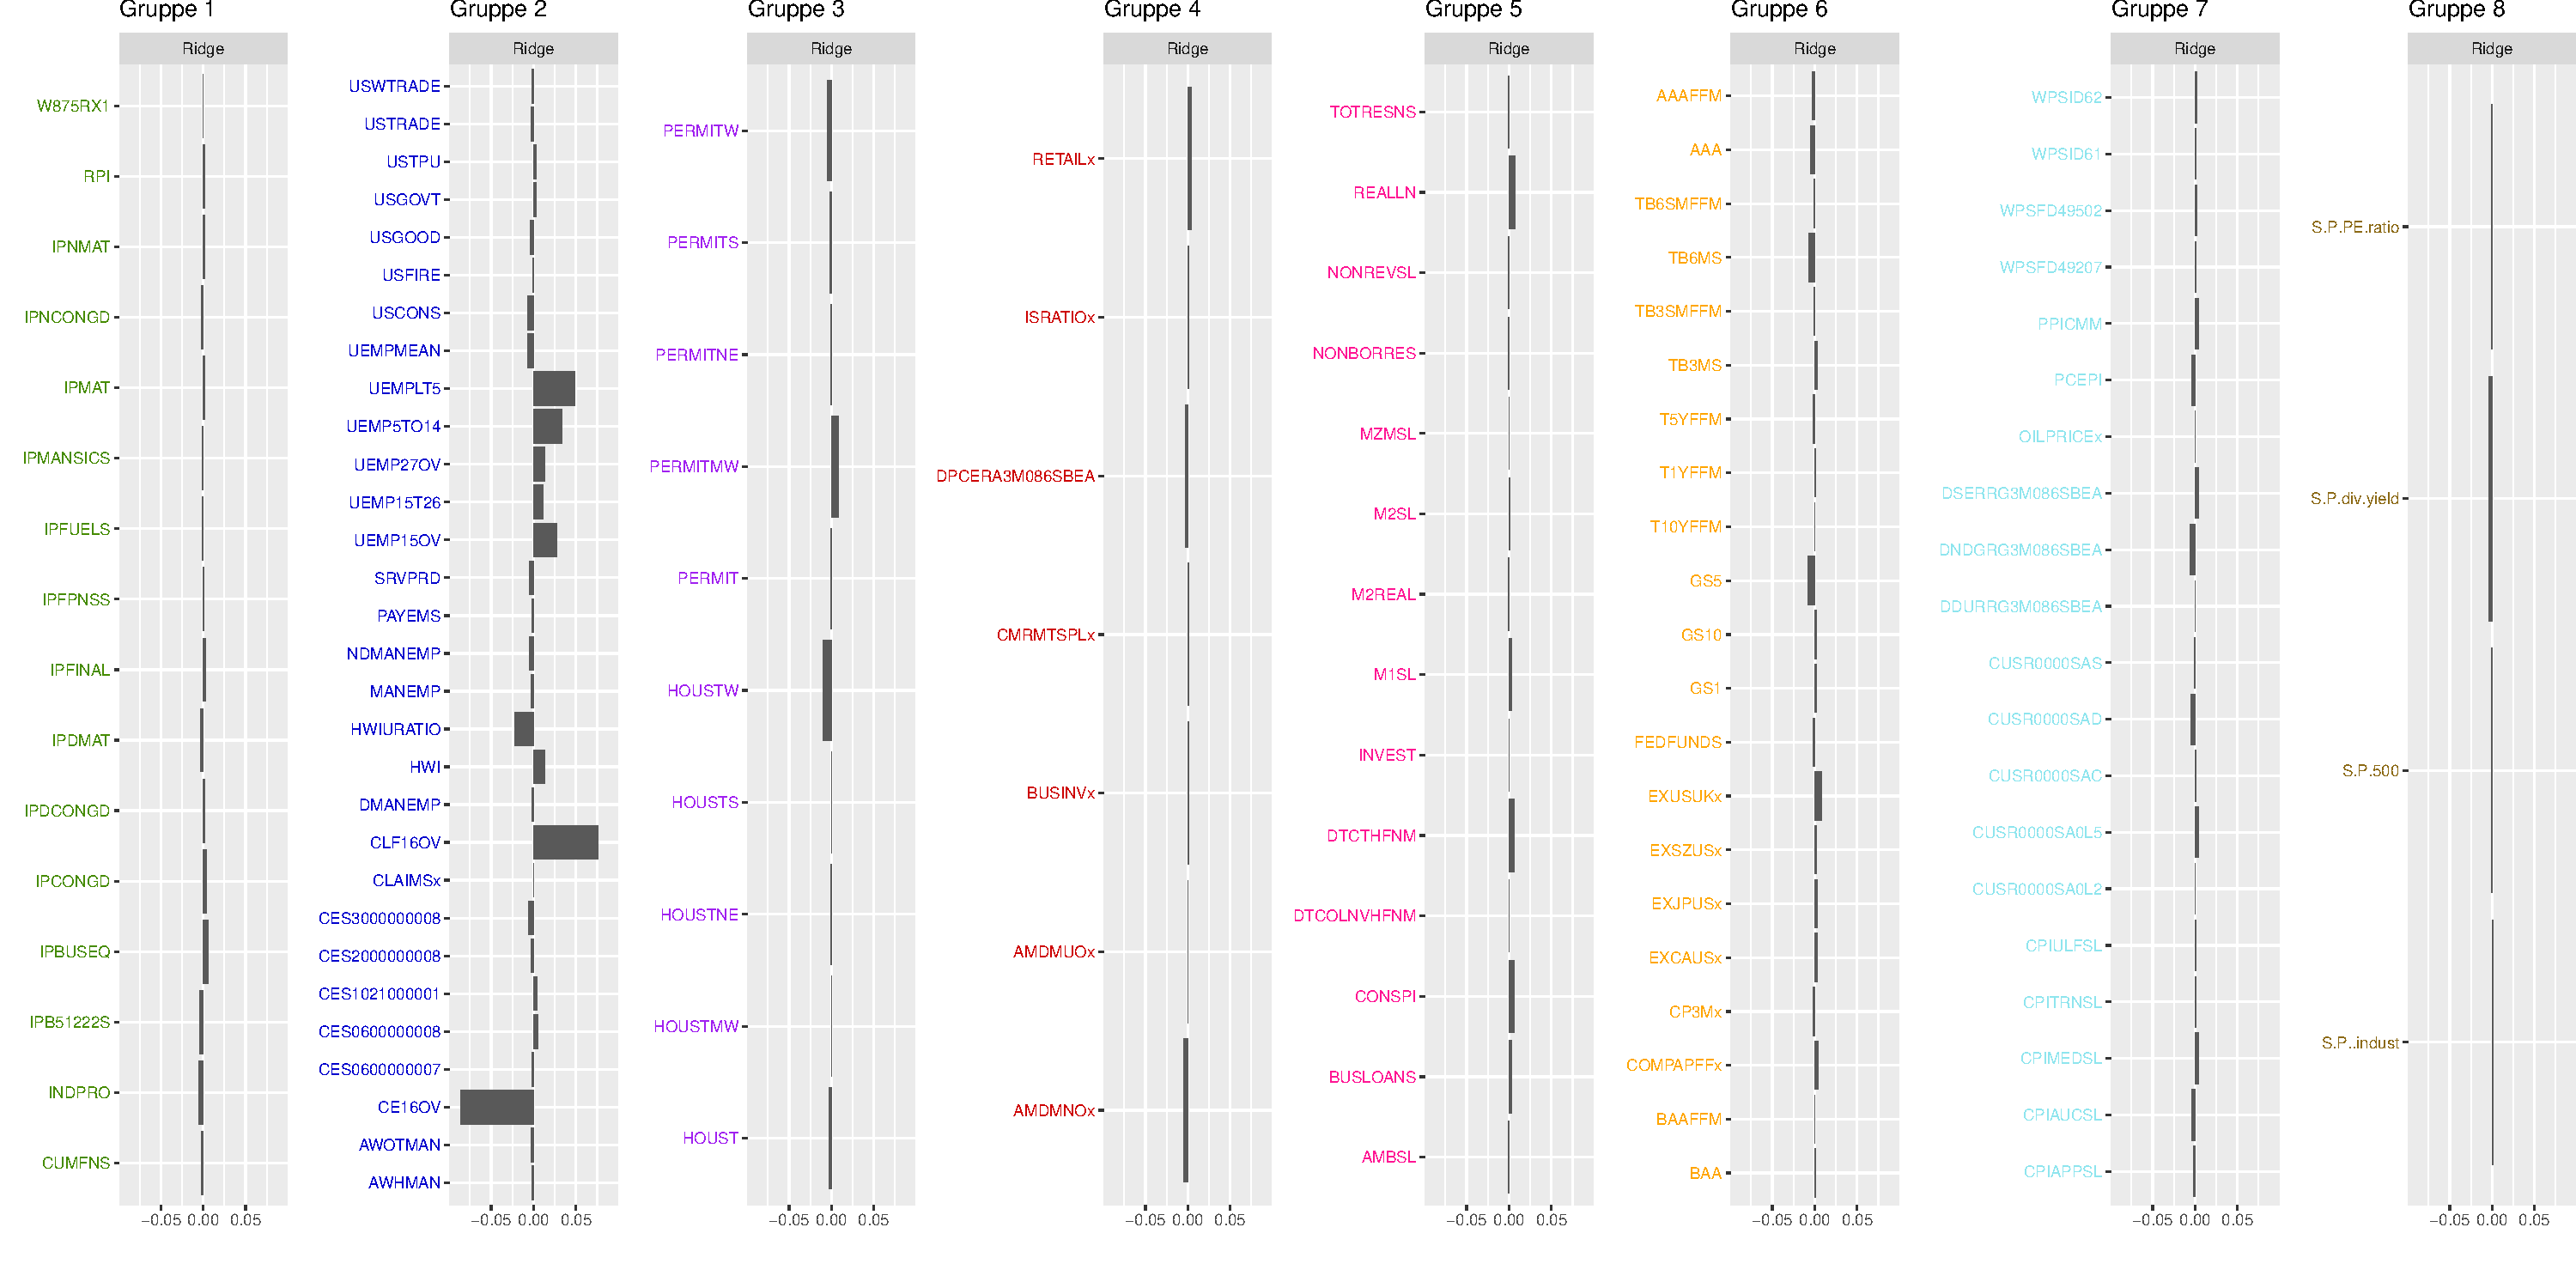
\includegraphics[width=1.5\textwidth]{fig/img/coef_ridge_kryds_coord.pdf}
		\caption{Estimerede koefficienter for ridge regression.}
		\label{fig:coef_ridge_kryds_coord}
\end{figure}
\end{landscape}

\begin{landscape}
\begin{figure}[htbp]
		\centering
		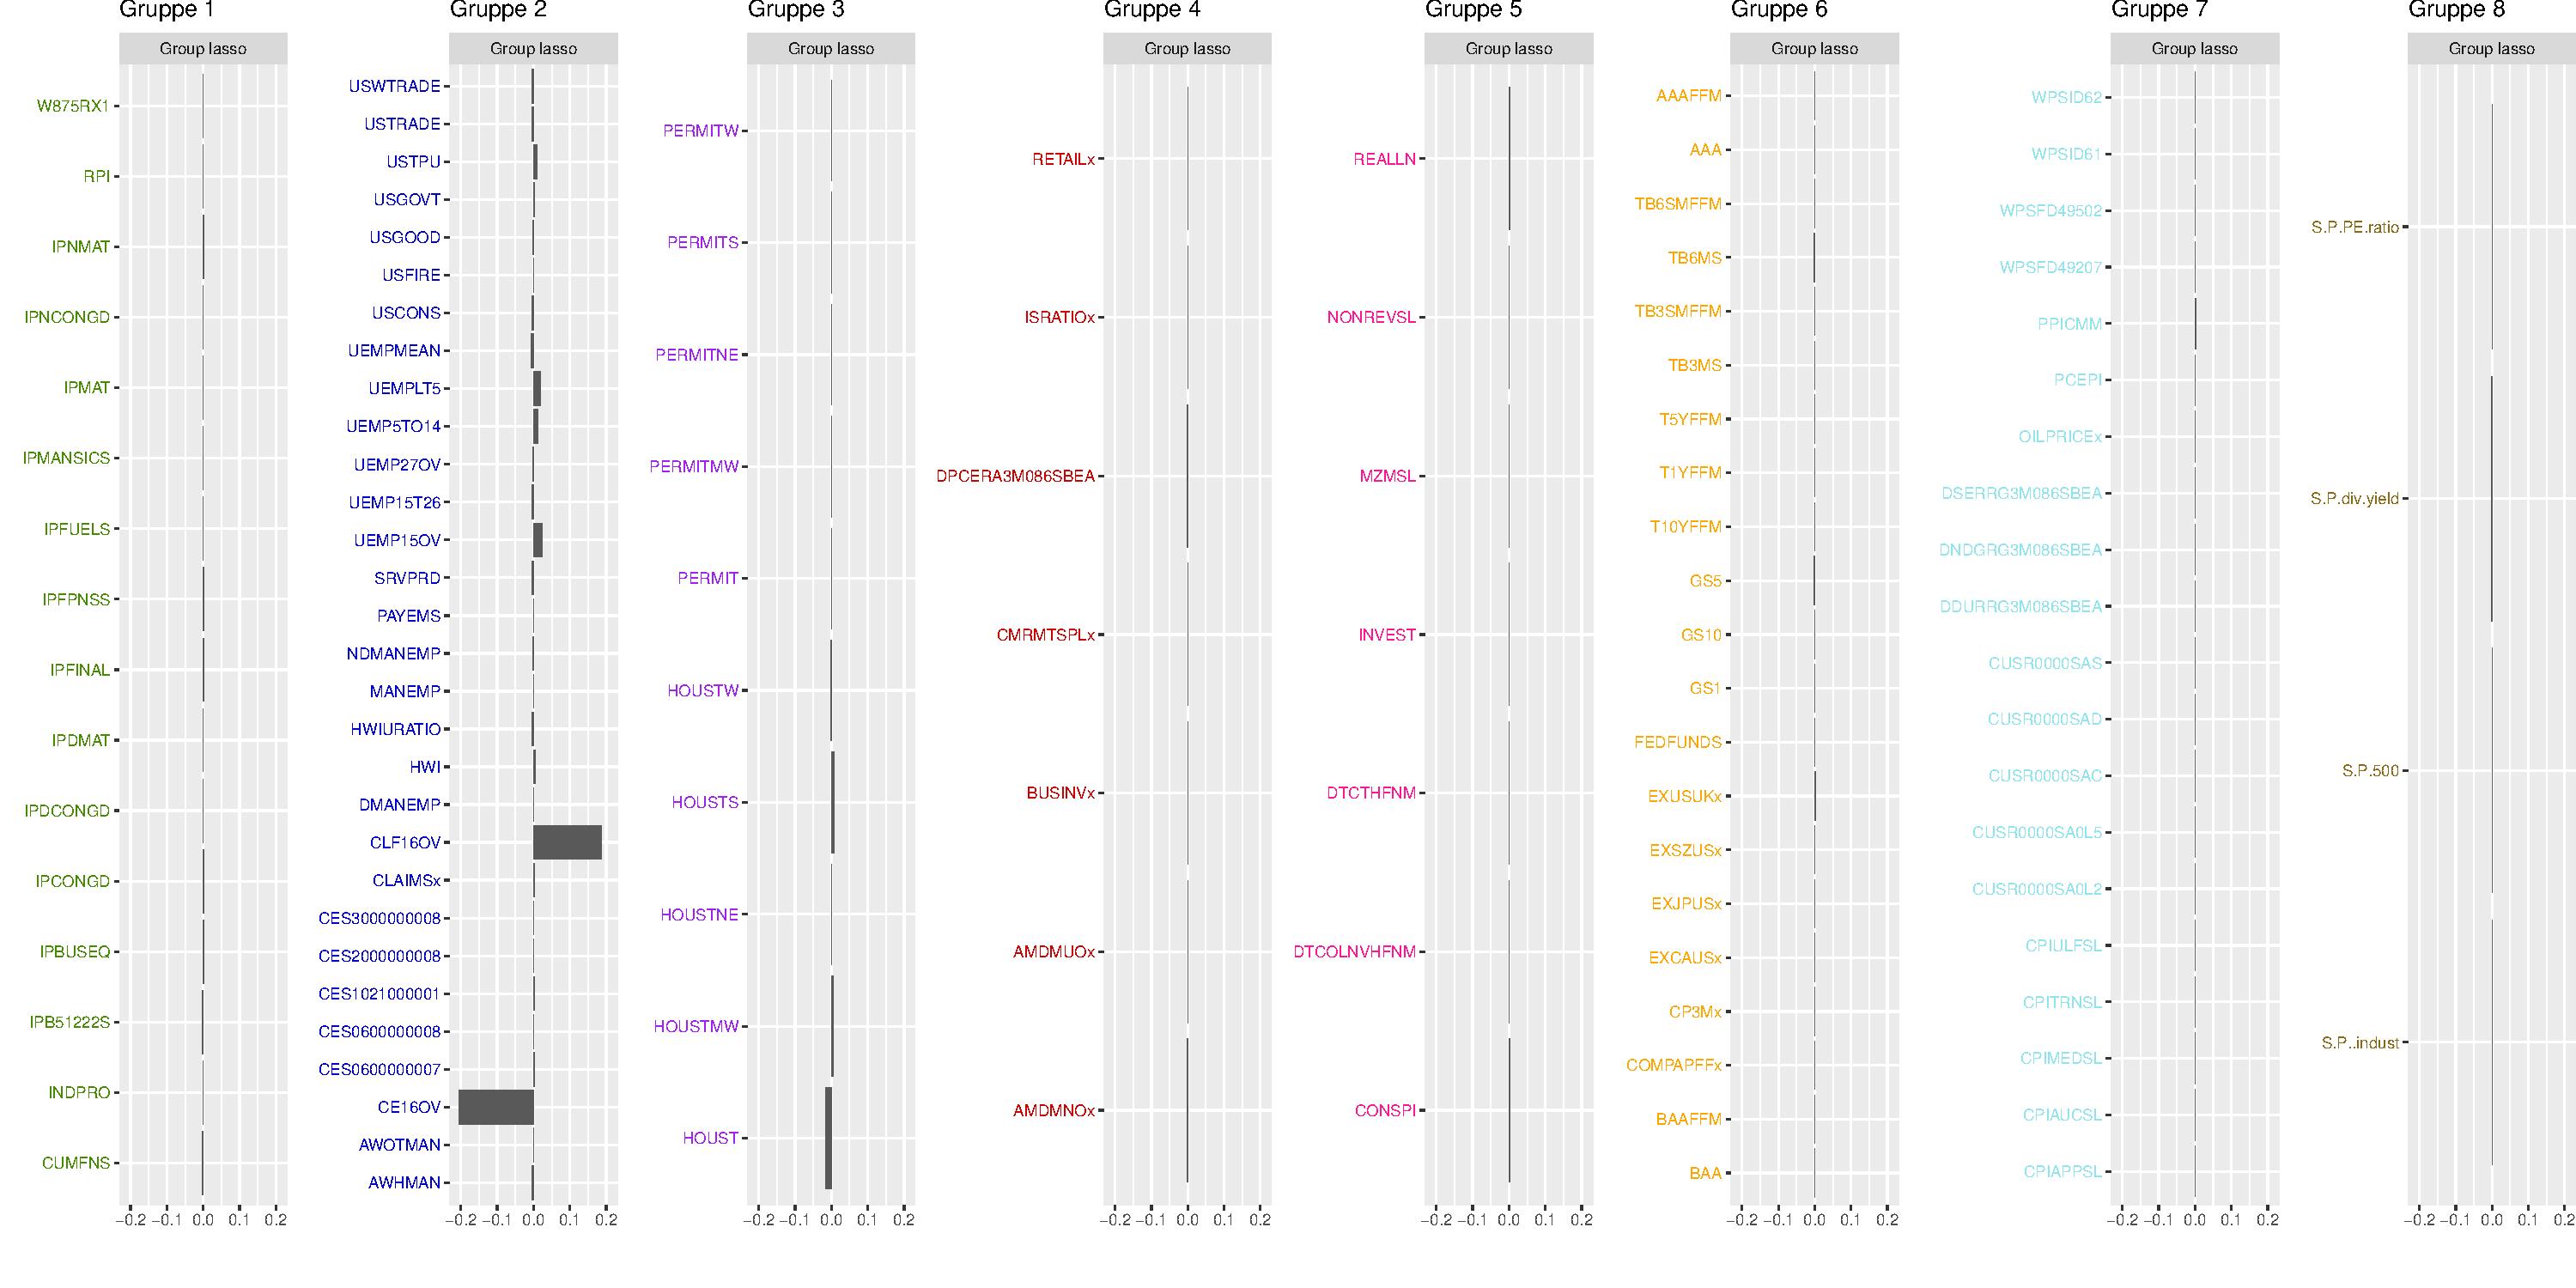
\includegraphics[width=1.5\textwidth]{fig/img/coef_gglasso_kryds_coord.pdf}
		\caption{Estimerede koefficienter for group lasso.}
		\label{fig:coef_gglasso_kryds_coord}
\end{figure}
\end{landscape}

\imgfigh{boxplot_lasso_coord_kryds.pdf}{1}{
Til venstre vises et boxplot af 1000 bootstrap realisationer af $\widehat{\tbeta}^{\text{lasso}} \del{{\widehat{\lambda}_\text{1sd}}} $, hvor $\widehat{\lambda}_\text{1sd}$ er estimeret ud fra krydsvalidering.  Plottet til højre illustrerer andelen af bootstrap realisationer, hvor parameter estimaterne er præcis lig nul.}{boxplot_lasso_coord_kryds}

%%%%% BIC %%%%%%%

\imgfigh{resid_lasso_coord_bic.pdf}{0.7}{Analyse af de standardiserede residualer for lasso  med optimeringsmetoden coodinate descent, hvor BIC  er brugt til at estimere $\widehat{\lambda}$. }{resid_lasso_coord_bic}

\imgfigh{resid_ridge_coord_bic.pdf}{0.7}{Analyse af de standardiserede residualer for ridge regression med optimeringsmetoden coodinate descent, hvor BIC  er brugt til at estimere $\widehat{\lambda}$. }{resid_ridge_coord_bic}

\imgfigh{resid_grp_coord_bic.pdf}{0.7}{Analyse af de standardiserede residualer for group lasso med optimeringsmetoden coodinate descent, hvor BIC  er brugt til at estimere $\widehat{\lambda}$. }{resid_grp_coord_bic}

\imgfigh{resid_adap_ols_coord_bic.pdf}{0.7}{Analyse af de standardiserede residualer for adaptive lasso med ols vægte med optimeringsmetoden coodinate descent, hvor BIC er brugt til at estimere $\widehat{\lambda}$. }{resid_adap_ols_coord_bic}

\imgfigh{resid_adap_lasso_coord_bic.pdf}{0.7}{Analyse af de standardiserede residualer for adaptive lasso med lasso vægte med optimeringsmetoden coodinate descent, hvor BIC  er brugt til at estimere $\widehat{\lambda}$. }{resid_adap_lasso_coord_bic}


\imgfigh{boxplot_lasso_coord_bic.pdf}{1}{Til venstre vises et boxplot af 1000 bootstrap realisationer af $\widehat{\boldsymbol{\beta}}^{\text{lasso}} \del{{\widehat{\lambda}}_\text{BIC}} $.
Til højere illustreret andelen af bootstrap realisationer, hvor parameter estimaterne er præcis nul}{boxplot_lasso_coord_bic}


%%%%% LARS kryds %%%%%%%
\imgfigh{lars_kryds_res.pdf}{0.7}{Analyse af de standardiserede residualer for LARS uden modifikation, hvor krydsvalidering  er brugt til at estimere $\widehat{s}$. }{lars_kryds_res}

\imgfigh{lars_lasso_kryds_res.pdf}{0.7}{Analyse af de standardiserede residualer for LARS med lasso modifikation, hvor krydsvalidering  er brugt til at estimere $\widehat{f}$. }{lars_lasso_kryds_res}

\imgfigh{boxplot_lars_kryds.pdf}{1}{Til venstre vises et boxplot af 1000 bootstrap realisatioer af $\widehat{\boldsymbol{\beta}}^{LARS} \del{\widehat{f}}$, hvor $\widehat{f}$ er estimeret ud fra krydsvalidering. Til højere illustreret andelen af bootstrap realisationer, hvor parameter estimaterne er præcis nul.}{coef_lars_kryds}


\imgfigh{boxplot_lasso_kryds.pdf}{1}{Til venstre vises et boxplot af 1000 bootstrap realisatioer af $\widehat{\boldsymbol{\beta}}^{lasso} \del{\widehat{f}}$, hvor $\widehat{f}$ er estimeret udfra krydsvalidering. Til højere illustreret andelen af bootstrap realisationer, hvor parameter estimaterne er præcis nul.}{coef_lasso_kryds}


\begin{table}
\center
\begin{tabular}{lcccc} 
\toprule
& LARS (CV) && lasso LARS  (CV) & LARS$_{TG}$ (CV) \\ \midrule
Skewness & -0.1222 && -0.1291 & -0.0792   \\
Kurtosis & -0.5251  && -0.5272 & 1.2576 \\
JB-test & 0.0241 &&  0.0217 & 0 \\
LB$_{10}$-test &0 && 0  & 0  \\  \bottomrule \toprule
& LARS (BIC) && lasso LARS (BIC) &  LARS$_{TG}$ (CV) \\ \midrule
Skewness & $-0.1606$  && $-0.1671$   & -0.1015 \\
Kurtosis &   $-0.4626$ && $-0.4344 $ & -0.4936  \\
JB-test & 0.0293 &&  $0.0353$ &  0.0428\\
LB$_{10}$-test & 0 && 0  & 0\\  \bottomrule 
\end{tabular}
\caption{Skewness, excess kurtosis, $p$-værdier for Jarque-Bera og Ljung-Box testen for de standardiserede residualer. Vi lader LB$_{10}$ betegne Ljung-Box test med lag = 10. } \label{tab:lars_kryds_res_tab}
\end{table}

%%%%% LARS bic %%%%%%%

\imgfigh{lars_bic_res.pdf}{0.7}{Analyse af de standardiserede residualer for LARS uden modifikation, hvor BIC  er brugt til at estimere $\widehat{s}$. }{lars_bic_resid}

\imgfigh{lars_lasso_bic_resid.pdf}{0.7}{Analyse af de standardiserede residualer for LARS med lasso modifikation, hvor BIC  er brugt til at estimere $\widehat{f}$. }{lars_lasso_bic_resid}

\imgfigh{boxplot_lars_bic.pdf}{1}{Til venstre vises et boxplot af 1000 bootstrap realisationer af $ \widehat{\boldsymbol{\beta}}^{LARS} \del{\widehat{f}}$, hvor $ \widehat{f}$ er estimeret ud fra BIC. Til højere illustreret andelen af bootstrap realisationer, hvor parameter estimaterne er præcis nul. }{boxplot_lars_bic}


\imgfigh{boxplot_lars_lasso_bic.pdf}{1}{Til venstre vises et boxplot af 1000 bootstrap realisationer af $ \widehat{\boldsymbol{\beta}}^{lasso} \del{\widehat{f}}$, hvor $ \widehat{f}$ er estimeret ud fra BIC. Til højere illustreret andelen af bootstrap realisationer, hvor parameter estimaterne er præcis nul. }{boxplot_lars_bic}

%\begin{table}
\center
\begin{tabular}{lccc} 
\toprule
& LARS && LARS med lasso modifikation \\ \midrule
Skewness & $-0.1606$  && $-0.1671$    \\
Kurtosis &   $-0.4626$ && $-0.4344 $ \\
JB-test & 0.0293 &&  $0.0353$ \\
LB$_{10}$-test & 0 && 0  \\  \bottomrule 
\end{tabular}
\caption{Skewness, excess kurtosis, p-værdier for Jarque Bera og Ljung Box teste for de standardiserede residualer fra LARS og LARS med lasso modifikation, hvor  $\widehat{s}$ og $\widehat{f}$ er valgt udfraBIC. Vi lader LB$_{10}$ betegne Ljung-Box test med lag = 10. } \label{tab:lars_bic_res_tab}
\end{table}





